\documentclass{article}
\usepackage{amsmath, amssymb, graphics, setspace}
\usepackage{graphicx}
\usepackage{tikz}
\usepackage{enumerate}
\usepackage{array}
\usepackage{float}
\usepackage{amsmath}
\usepackage{geometry}
\usepackage{pdfpages}
\usepackage{latexsym}
\usepackage{multicol}
\usepackage{geometry}
\usepackage{booktabs}
\usepackage{graphicx}
\usepackage{subfigure}
\usepackage{upgreek}
\usepackage{multirow}
\usepackage{indentfirst}
\usepackage{color}
\usepackage{bm}
\usepackage{caption}
\usepackage{amstext}
\usepackage{natbib}
\usepackage[colorlinks,linkcolor=blue]{hyperref}
\renewcommand{\baselinestretch}{1.5}
\geometry{left=2.5cm, right=2.5cm, top=2cm, bottom=2cm}
\title{\Huge {Donut.c}}
\author{Group 2 \\ \\
Pingbang Hu ID: 519370910026 \\
Xiaoyu Chen ID: 519370910020 \\
Jinyi Wu ID: 519021910005}
\date{18 April 2021}
\begin{document}

\maketitle
%--------------------------------------------------------------------Introduction----------------------------------------------------------------------------------------------------------------------
\section{Introduction}

\par 3D computer graphics are graphics that use the 3D model in computer to render and generate 2D images. 
Nowadays, the resolution of the 3D computer graphics becomes higher and higher, even the material of the model and the effects of light can also be simulated.

\par We are interested in the most basic mechanism of 3D computer graphics. 
We want to figure out how 3D model is built and stored inside the computer, what is the algorithm to move the model and how to render 2D images from a 3D model.

\par Back to 2006, there's an interesting C project on the internet called Donut.c, which can print the ascii characters in the terminal of a rotating donut. 
And recently it is widely spread and discussed through the internet, and after we look into the source code, we find out that the whole algorithm is based on what we have learned in Vv214. 
From here, we want to do some deep research and expand this project based on the current one.

\begin{figure}[H]
  \centering
  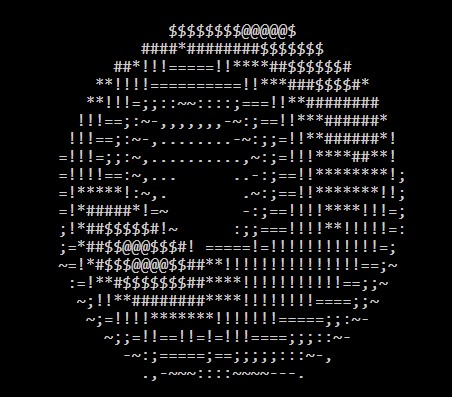
\includegraphics[width=0.4\textwidth]{Figures/donut.jpg}
  \caption{The donut}
\end{figure}

%--------------------------------------------------------------------Relation to Linear Algebra--------------------------------------------------------------------------------------------------------
\section{Relation to Linear Algebra}

\par The program first draws a circle on a 3D x-y-z coordinate, then, rotates the circle around the central axis of the donut, which will create a donut in 3D space.
It is noticed that the algorithm only draws the shell of the donut. 
However, it does not matter because our final goal is to render it into 2D images and the donut's shell can not transmit light. 
Next, it chooses the position of the viewer and applies projection matrix on every point of the donut to generate a 2D image.
Finally, according to the normal vector of each point, the program calculates the light reflection through dot product. 
The image of the donut is shown by different ASCII characters and the 'size' of ASCII characters represents the brightness of the point.

\par In this program, the following linear algebra methods are used:

\begin{enumerate}
  \item Linear Transformation : Rotation Matrix in 3 dimensional space.
  \item Orthogonality : Produce normal vector from a surface.
  \item Inner product : Dot product of normal vector and light vector to get the brightness.
  \item Projection : Produce 2d animation from 3d space.
  \item Discrete Dynamic System : Compute the next frame by the current state of this system(the donut).
\end{enumerate}

%--------------------------------------------------------------------Goals and Expected Results--------------------------------------------------------------------------------------------------------
\section{Goals and Expected Results}

\par Our goal is to get the total understanding of the basic concept of 3D computer graphics, and from here, we can modify it to generate different kinds of animation. 
For example, we can change the shape, the size, the rotating speed, or even the dimension of the object to show a 4-dimension 'cub'.

%--------------------------------------------------------------------Reference-------------------------------------------------------------------------------------------------------------------------
\section{Reference}

\begin{enumerate}
  \item \url{https://www.a1k0n.net/2011/07/20/donut-math.html}
  \item \url{https://en.wikipedia.org/wiki/3D_computer_graphics}
  \item \url{https://www.javatpoint.com/computer-graphics-z-buffer-algorithm}
\end{enumerate}

%--------------------------------------------------------------------Workload Distribution-------------------------------------------------------------------------------------------------------------
\section{Workload Distribution}
\begin{itemize}
  \item Hu Pingbang : Slides making
  \item Chen Xiaoyu : Coding.
  \item Wu Jinyi : Presenting.
\end{itemize}

\end{document}